\chapter*{Classification}
\addcontentsline{toc}{chapter}{Classification}
Schaefer \etal \cite{schaefer_name_2011} were able to use the unique time course of the component responsible for the most variance to differentiate between stimuli.
Analyzing our components we have not yet been able to reproduce this significant stimulus classification accuracy. 
This could be caused by our much smaller number of trials which are substantially longer than those used by \cite{schaefer_name_2011}. 
On average we used \hl{X number of} trials in our analysis, while Schaefer et al. (2011) collected 145 trials of each of their stimuli.

We then attempted a different approach to classification using machine learning techniques. This approach facilitates better pattern learning by adapting components linked across subjects but that are also specific to each individual subject. 
We trained a \ac{CAE} as described in \cite{masci_stacked_2011} and implemented using pylearn2 \cite{goodfellow_pylearn2_2013}.
%CAEs are a special variant of a \ac{CNN} that encode their input using convolution into a compressed internal representation which is then decoded using de-convolution into the original space trying to minimize the reconstruction error. 
%Such a neural network can be used to learn a meaningful but compressed representation of the data. 
In this case the 64 \ac{EEG} channels were reduced to four combined channels -- each computed by a separate convolution filter. 
%These filters are very similar to the components produced in \ac{PCA} and \ac{ICA}. 
%The difference is the objective that is used to compute these components. 
%The \ac{CAE} filters aim to minimize the \ac{MSRE} using stochastic gradient descent over mini-batches rather than the orthogonality or independence criteria used in \ac{PCA} and \ac{ICA} respectively. 
\subsection*{Perception Classification Results}
First the \ac{CAE} was trained on all trials in the perception condition. The learned filter weights were then used as initialization values to create individual \ac{CAE}s specific to each participant.
The filters can be seen in \autoref{fig:components}. 
Minor differences between subjects can be seen. 

\begin{figure}[t]
  \begin{center}
    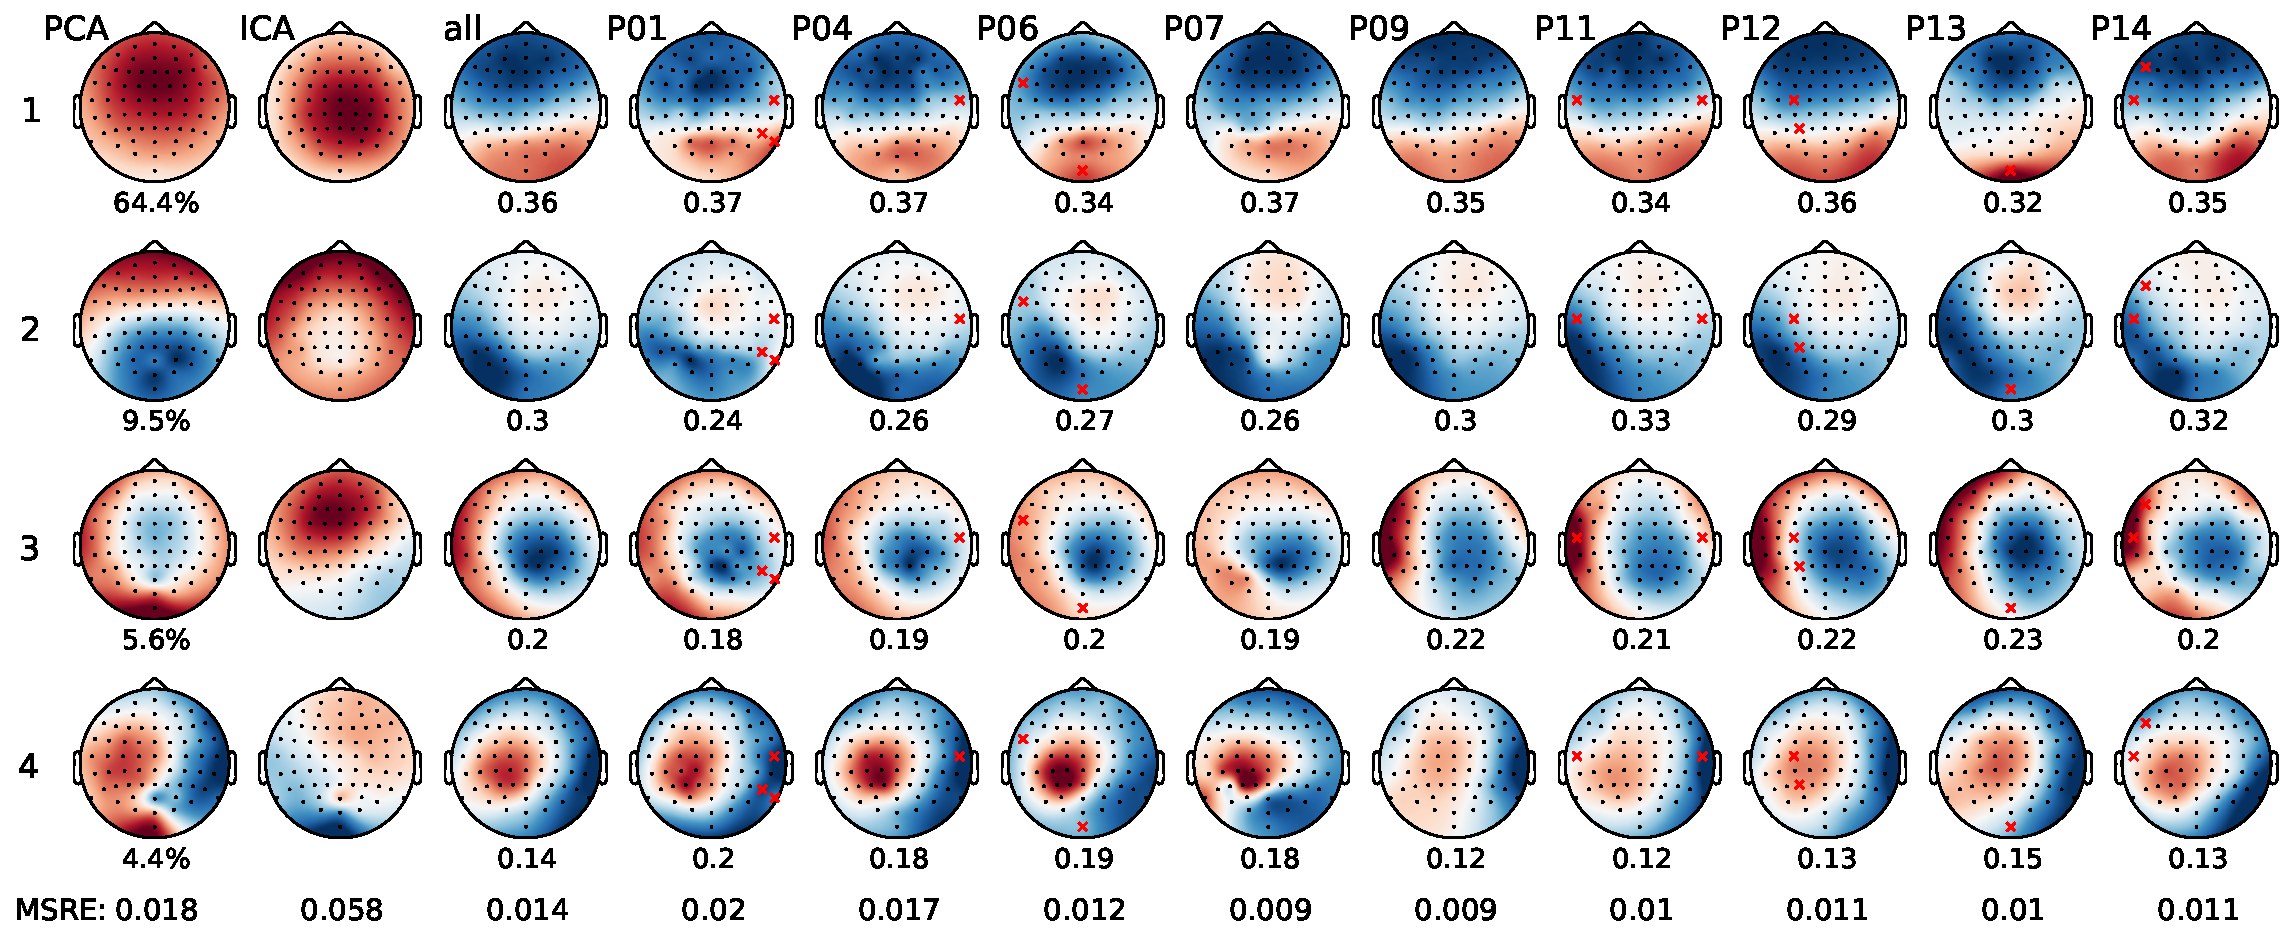
\includegraphics[width=\columnwidth,keepaspectratio=true]{Figures/topoplots_all.pdf}
    \caption{
Topographic map visualization of the EEG channel weights for the top 4 signal components derived from the perception trials. The leftmost two columns show the top 4 principal components (explaining over 87\% of the variance in total) and the corresponding independent components computed using extended Infomax ICA. The remaining columns show the weights learned by the convolutional auto-encoder for all subjects combined (third column) and all individual subjects labeled P01 to P14 accordingly. Numbers below the plots refer to the percentage of explained variance for principal components and the normalized biases for the filters of the convolutional auto-encoder respectively. Noisy EEG channels that were removed and interpolated are marked by red X?s. For subjects P09 to P14, mastoid channel referencing was applied. Values at the bottom of each column refer to the mean squared reconstruction error (MRSE) per sample.
}
    \label{fig:components}
  \end{center}
\end{figure}

We used the data from the learned components to train simple \ac{CNN}s with a single convolution layer and a \hl{DLSVM output layer} \cite{tang_deep_2013} on two classification tasks: stimulus identification (12 classes) and time-signature recognition (2 classes). 
We trained the CNN on 60\% of the trials. This same training set was used to train the \ac{CAE} prior to the \ac{CNN} training. 
The best model was selected using a validation set (20\% of trials) and it was evaluated on a test set (20\% of trials). 
\hl{We used dropout regularization} \cite{hinton_improving_2012}, momentum, and a linear learning rate decay over epochs.
A simple \ac{CNN} that used 16 [1x4]-convolution filters (over 1 sample in all 4 component activation channels) obtained 65.8\% (p=0.05) accuracy on the binary time-signature classification task. 
A CNN using 1 [16x4]-convolution filter (over 250ms in all 4 component activation channels with pooling for 140ms-windows and 5x sub-sampling obtained 19.5\% (p=0.001) on the 12 class stimulus recognition task. 
Significance values were determined by using the cumulative binomial distribution to estimate the likelihood of observing a given classification rate by chance.

\subsection*{Imagination Classification Results}
Imagination results from CNN. 

Table to summarize all results? 
